
\section{Personnages}
\lettrine{L}{e} c\oe{}ur des jeux de rôle réside dans la possibilité de créer, améliorer et faire évoluer son propre personnage. Voilà comment ça fonctionne dans {\jedifont Starwars reloaded}. 

\subsection{Les Attributs}
Chaque personnage commence le jeu avec d4 dans chaque Attribut et dispose de 5pt pour les améliorer. Améliorer l'un d'entre eux d’un type de dé (par exemple, de d4 à d6) coûte 1 point avec une limite : vous ne pouvez aller au-delà du d12.

\subsection{Compétences}
Les Compétences représentent les aptitudes apprises comme le Tir, le Combat, les connaissances professionnelles ou scientifiques et ainsi de suite. Elles sont générales et englobent tous les aspects qui leur sont reliés. Par exemple Tir englobe les fusils, les arcs, les lance-roquettes et toutes les armes à distance. Vous disposez de 15 points à répartir entre vos Compétences. Chaque dé de Compétence coûte 1 point (en commençant à d4) tant qu’il est inférieur ou égal à l’Attribut dont il dépend (noté entre parenthèses près du nom de la Compétence). Chaque dé de Compétence supérieur à l’Attribut dont il dépend coûte 2 points. De même que pour les Attributs, aucune Compétence ne peut dépasser d12.

\subsection{Races Jouable}
% To be balanced correctly, all race most have CAP +2
Vous pouvez choisir pour votre personnage n’importe quelle race disponible dans l'univers de Starwars. 

\subsubsection{Humain}
\begin{flushright}
\begin{tabular}{ l l }
	\textbf{Type} 			& Humanoïde \\
   	\textbf{Planète} 		& Terre \\
   	\textbf{Language} 		& Basic \\
   	\textbf{Orientation} 	& Neutre \\
\end{tabular}
\vspace{-60}
\end{flushright}


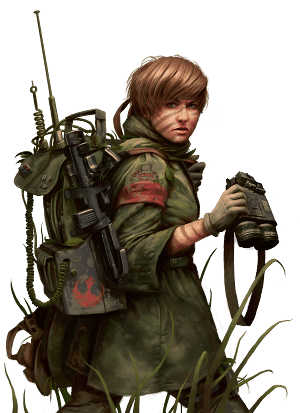
\includegraphics[width=5cm]{img/races/humain.png} 

Cette race comprend aussi bien les humains au sens strict (qu’ils soient originaires de Coruscant, de Correlia, de Kuat, de Naboo...) que les humanoïdes dont les caractéristiques physiques, intellectuelles, sociales et culturelles sont suffisamment proches de celles des humains pour qu’il soit possible de les assimiler en termes de jeu. Cela inclut par exemple les iridoniens (zabraks) et les dévaroniens.

\begin{description}[align=left]
\item [Adaptabilité] 	CAP +2
	Les humains sont une race pleine de ressources, ils s'adaptent rapidement à toutes sorte de difficultés ou environnements.\\
	\emph{Compétence à d6}
\end{description}

\subsubsection{Barabel}

\begin{flushright}
\begin{tabular}{ l l }
	\textbf{Type} 			& Reptile \\
   	\textbf{Planète} 		& Barab I \\
   	\textbf{Language} 		& Barabel \\
   	\textbf{Orientation} 	& Obscur \\
\end{tabular}
\end{flushright}

\vspace{-50}
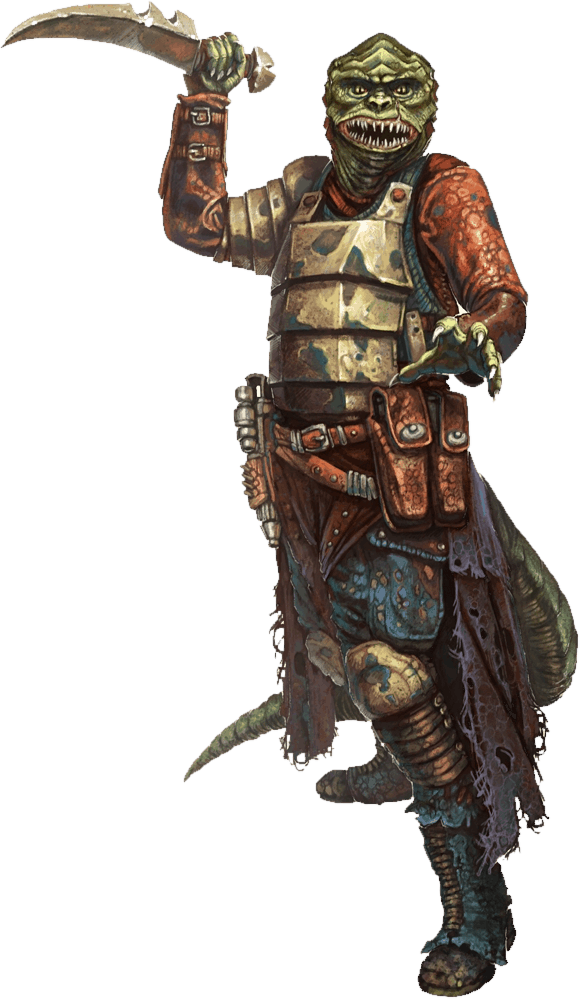
\includegraphics[width=5cm]{img/races/barabel.png}

Originaire de Barab I, les Barabels sont resté une race relativement primitive et isolée. Les Barabels vivent en clans dans un société principalement matriarcale. Ils sont fasciné par la guerre, la violence et les armes. Les Barabels ne sont pas profondément cruels mais il restent agressif de nature. En raison des nombreux rituels précédent les négociations, la diplomatie avec les Barabels est un exercice compliqué.

Le Barabel adulte est un reptile bipède dont la taille dépasse toujours les deux mètres. Sa dentition est formée d'une multitude de dents en forme d'aiguilles qui peuvent atteindre jusqu'à cinq centimètres de long et ses mains sont équipées de griffes puissantes.

\begin{description}[align=left]
\item [Enfance difficile] 	% CAP +1 +1
		De par l'environnement hostile de leur planète natale, les Barabels possèdent une résistance accrue à la chaleur et aux radiations.\\
		\emph{+4 en Résistance à la chaleur}\\
		\emph{+4 en Résistance aux radiations}
\item [\OE{il} Ophidien] 	% CAP +1
		Les yeux ophidiens du Barabel lui permettent de capter la plupart des ondes lumineuses allant du jaune à l'infrarouge mais il confond facilement les couleurs tirant dans les bleus et violets.\\
		\emph{Infravision}
\item [Arme naturelle]		% CAP +1
		Les mains des Barabels sont équipé de puissante griffes.\\
		\emph{For + d6 de dégâts}
\item [Balayage]			% CAP +2
		Les Barabels utilise leur appendice caudal d'instinct dans les combats.\\
		\emph{+ Atout Balayage}
\item [Primitif]			% CAP -3
		Les Barabels sont une race encore primitive.\\
		\emph{Int <= d6}
\item [Dur d'oreille]		% CAP -1
		Les Barabels en tant que reptilien ne possède pas d'oreille, il entendent par vibrations.\\
		\emph{Dur d'oreille (Mineur)}
\end{description}


\subsubsection{Bothan}

\begin{flushright}
\begin{tabular}{ l l }
	\textbf{Type} 			& Félin \\
   	\textbf{Planète} 		& Bothawui \\
   	\textbf{Language} 		& Bothese \\
   	\textbf{Orientation} 	& Lumineux \\
\end{tabular}
\end{flushright}

\vspace{-55}
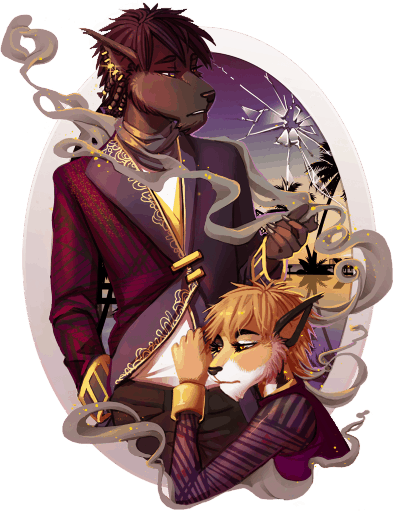
\includegraphics[width=5cm]{img/races/bothan.png}

Les Bothans sont des humanoïdes trappus, dont le corps est recouvert d'une épaisse fourrure pouvant varier du blanc-cassé à brun très foncé.
Le peuple bothan est originaire de la planète Bothawui, un monde cosmopolite épargné des troubles de la Guerre Civile Galactique en raison de la neutralité officielle du gouvernement bothan. Plusieurs colonies ont également été construites sur des planètes proches, telles que Kothlis, qui est désormais le siège d'une importante communauté. Toutes ces colonies forment l'Espace Bothan.\\
La structure sociale des Bothans est constituée par des clans familiaux, dont le nom est inclus dans le nom de chaque Bothan, à la suite d'une apostrophe.

\begin{description}[align=left]
\item [Agilité du Félin] 			% CAP +2
		Les Bothans possède la grace de leur ancêtres félins.\\
		\emph{Commence avec d6 Agi}
\item [Service de renseignement] 	% CAP +1
		Depuis plus de 300 ans ces êtres intelligents et rusés ont perfectionné leurs façons de faire, et ont développé un vaste réseau d'espions et d'informateurs destiné à recueillir toutes sortes d'informations sur les sujets les plus importants.\\
		\emph{d6 en Réseaux}
\item [Comme en plein jour] 		% CAP +1
		Grace à leur yeux de félins, les Bothans voient parfaitemnet dans l'obscurité.\\
		\emph{Vision Nocture}
\item [Déplacement rapide] 			% CAP +2
		Les Bothans, s'ils se baissent sur leur quatres pattes peuvent atteindre des vitesses de 80km/h.\\
		\emph{All = 10}
\item [Frêle] 						% CAP -2
		De contitution moins résistante, les Bothans sont moins adapté aux combats rapproché.\\
		\emph{-1 Résistance}
\item [Mauvaise réputation] 		% CAP -1
		Les ruses conduites par ce peuple, ainsi que l'opacité inhérente au Réseau Bothan, ne jouent pas en leur faveur. Certains leur reprochent de ne pas avoir prévu que l'Empire tendait une embuscade aux forces de l'Alliance.\\
		\emph{\'Etranger}
\item [Prudent] 					% CAP -1
		Les Bothans ne font rien à la légère, ils ne laissent nulle place au hazard et chaque décision est murrement réfléchie. Ils ne connaissent pas l'urgence.\\
		\emph{Prudent}
\end{description}

\subsubsection{Chiss}
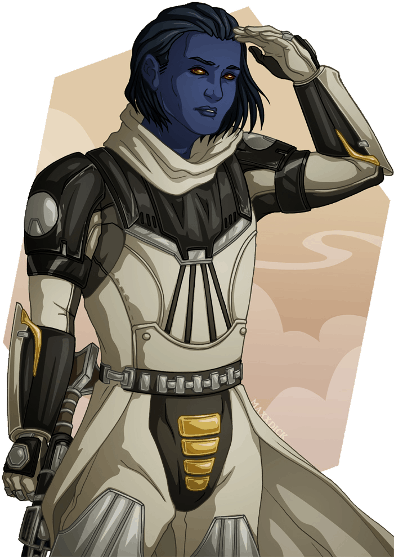
\includegraphics[width=5cm]{img/races/chiss.png}

\vspace{-80}

\begin{flushright}
\begin{tabular}{ l l }
	\textbf{Type} 			& Humanoïde \\
   	\textbf{Planète} 		& Csilla \\
   	\textbf{Language} 		& Cheunh \\
   	\textbf{Orientation} 	& Obscur \\
\end{tabular}
\end{flushright}

\vspace{15}

Les Chiss font en moyenne 1,80m et ont une morphologie humaine. Cependant, il est impossible de les confondre à cause de leur peau bleue et de leurs yeux d’un rouge éclatant. Ils ont toujours des cheveux noirs, bien qu’avec les années, certains voient des cheveux blancs apparaitre. \\ 

La société Chiss est très évoluée. Ils ont de l’intérêt pour les arts et la science et maintiennent une puissante force militaire. Ils ont la réputation d’être de fins stratèges militaires mais leur façon de penser se retrouve dans tous les domaines de la vie quotidienne. Ils réfléchissent et pensent à différents points de vue et aux alternatives lorsqu’ils doivent prendre une décision.  

\begin{description}[align=left]
\item [Charismatique] 			% CAP +2 +2 +1
		Les Chiss sont des êtres charismatique habitué à commander des armées.\\
		\emph{+2 Cha}\\
		\emph{Commandement}\\
		\emph{d6 Connaissance (Combats)}
\item [Aquité visuelle] 		% CAP +1
		Les modifications qu’ont subies leurs yeux leur ont également donné une plus grande acuité visuelle.\\
		\emph{d6 Perception}
\item [Arrogant] 				% CAP -2
		Les Chiss sont fréquemment perçus par le reste de la galaxie, comme un peuple arrogant, calculateur et distant.\\
		\emph{Arrogant}
\item [Insensible à la Force] 		% CAP -1
		Les Chiss ne sont pas connus pour être une espèce sensible à la Force. Ils n’ont eut qu’un seul exemple d’individu sensible, en la personne de Sev’rance Tann. Cette dernière avait optée pour le côté obscur.\\
		\emph{A la création, l'augmentation de l'\^Ame coute 2pt}
\end{description}

\subsubsection{Droïde}
\vspace{4\baselineskip}
\begin{tabular}{ l l }
	\textbf{Type} 			& Artificiel \\
   	\textbf{Planète} 		& Multiple \\
   	\textbf{Language} 		& Binaire \\
   	\textbf{Orientation} 	& Neutre \\
\end{tabular}

\vspace{-11\baselineskip}

\begin{flushright}
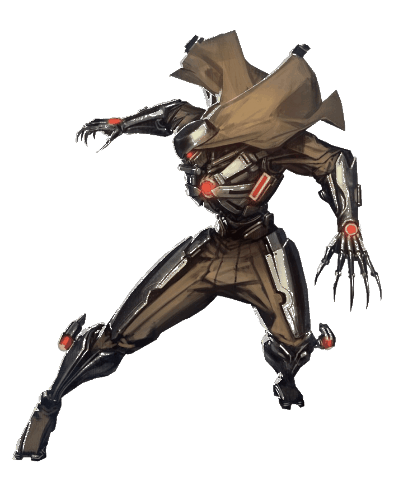
\includegraphics[width=6cm]{img/races/droide.png}
\end{flushright}
\vspace{-2\baselineskip}

Les Droïdes ne sont pas une race à proprement parlé mais des entités artificielles créés par d'autres races. Il peuvent être de Combat, de Protocole, de Compagnie, \ldots 
De par leur état les Droïde ne peuvent et ne pourront jamais utiliser la Force, c'est une notion qui leur est totalement étrangère.

\begin{description}[align=left]
\item [Charismatique] 			% CAP +2 +2 +1
		Les Chiss sont des êtres charismatique habitué à commander des armées.\\
		\emph{+2 Cha}\\
		\emph{Commandement}\\
		\emph{d6 Connaissance (Combats)}
\item [Aquité visuelle] 		% CAP +1
		Les modifications qu’ont subies leurs yeux leur ont également donné une plus grande acuité visuelle.\\
		\emph{d6 Perception}
\item [Arrogant] 				% CAP -2
		Les Chiss sont fréquemment perçus par le reste de la galaxie, comme un peuple arrogant, calculateur et distant.\\
		\emph{Arrogant}
\item [Insensible à la Force] 		% CAP -1
		Les Chiss ne sont pas connus pour être une espèce sensible à la Force. Ils n’ont eut qu’un seul exemple d’individu sensible, en la personne de Sev’rance Tann. Cette dernière avait optée pour le côté obscur.\\
		\emph{A la création, l'augmentation de l'\^Ame coute 2pt}
\end{description}

\subsubsection{Gungan}
\subsubsection{Sullustain}
\subsubsection{Togruta}
\subsubsection{Twl'lek}
\subsubsection{Wookie}
\subsubsection{Zabrak}

\newpage % Acts as columbreak because of twocolumn option; for pagebreak use \clearpage

% For more columns, you can say \begin{dndtable}[your options here}.
% For instance, if you wanted three columns, you could say
% \begin{dndtable}{XXX}. The usual host of tabular parameters are
% aailable as well.
\header{Nice table}
\begin{dndtable}
   	\textbf{Table head}  & \textbf{Table head} \\
   	Some value  & Some value \\
   	Some value  & Some value \\
   	Some value  & Some value
\end{dndtable}

\begin{paperbox}{Do the Players need direction?}
	\lipsum[1]
\end{paperbox}

% You can optionally not include the background by saying
% begin{monsterboxnobg}
% \begin{monsterbox}{Monster Foo}
% 	\textit{Small metasyntatic variable (golbinoid), neutral evil}\\
% 	\hline
% 	\basics[%
% 	armorclass = 12,
% 	hitpoints  = 16 (3d8 + 3),
% 	speed      = 50 ft
% 	]
% 	\hline
% 	\stats[
%     STR = \stat{12}, % This stat command will autocomplete the modifier for you
%     DEX = \stat{7}
% 	]
% 	\hline
% 	\details[%
% 	% If you want to use commas in these sections, enclose the
% 	% description in braces.
% 	% I'm so sorry.
% 	languages = {Common Lisp, Erlang},
% 	]
% 	\hline \\[1mm]
% 	\begin{monsteraction}[Monster-super-powers]
% 		This Monster has some serious superpowers!
% 	\end{monsteraction}
% 	\monstersection{Actions}
% 	\begin{monsteraction}[Generate text]
% 		This one can generate tremendous amounts of text! Though only when it wants to.
% 	\end{monsteraction}
% 
% 	\begin{monsteraction}[More actions]
%     See, here he goes again! Yet more text.
% 	\end{monsteraction}
% \end{monsterbox}
